\documentclass[11pt, letterpaper]{article}
\setlength{\parindent}{0in}
\setlength{\textheight}{8.7in}
\setlength{\textwidth}{6.8in}
\setlength{\oddsidemargin}{-0.3in}
\setlength{\evensidemargin}{0.0in}
\addtolength{\topmargin}{-1in}
\setlength{\parskip}{0.1in}

\usepackage{amsmath, amsfonts, color}
\usepackage{bm}
\usepackage{enumerate}
\usepackage{graphicx}
\usepackage{pdflscape}
\usepackage{afterpage}
\usepackage{capt-of}
\usepackage{hyperref}
\usepackage{color}
\newcommand*{\justifyheading}{\raggedleft}

\usepackage[top=1in, bottom=1.25in, left=1.25in, right=1.25in]{geometry}



\begin{document}

\Large 
\begin{center}
\bf Ferry Curious about WSDOT Sailing Times \\
\bf Mike Logsdon and Zach Stednick
\end{center} 
\normalsize 


Although coverage of transit often revolves around Metro or Sound Transit, we wanted to shift the focus a bit to look at another method - ferries. It seems that the majority of the coverage of WSDOT ferries focuses on the fiscal side such as costs of ferry maintenance and replacement as well was critical examinations of ferry employee salaries.
We wanted to shift the conversation slightly and focus on the logistical aspect of the ferry system. Are the ferries generally on time? Are certain routes or vessels unusually punctual or unusually late? Are some days or times better or worse than others? To achieve this we filed a Public Records Request to gain access to this data. Here we present findings for on-time rates for calendar year 2014, where we specifically investigated the difference between actual and scheduled departure times. For simplicity this report considers only Puget Sound ferry routes. This work considers the data in an exploratory fashion -- investigating patterns in the data but not yet considering statistical models or prediction algorithms.

\begin{figure}
\begin{center}
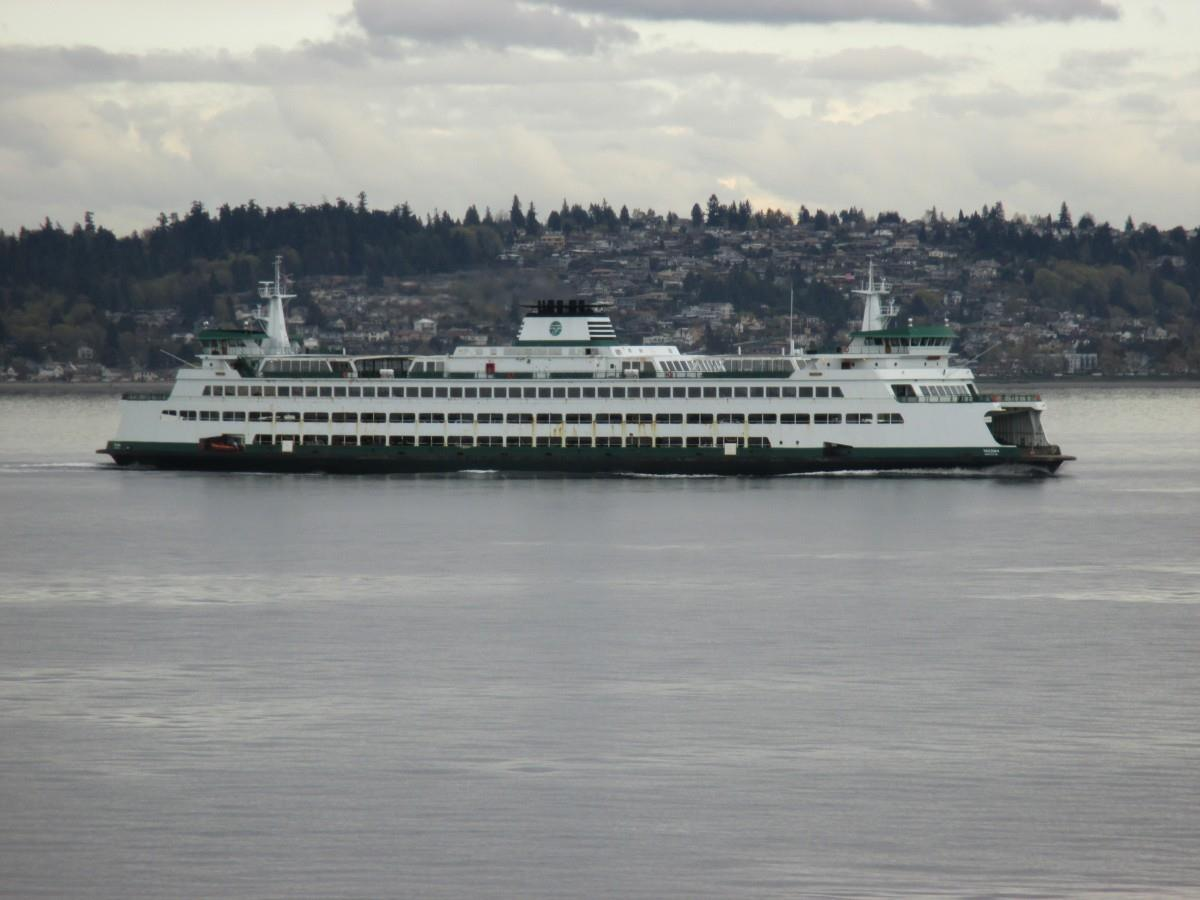
\includegraphics[scale = .4]{ferry.jpg}
\end{center}
\end{figure}

\section*{Summary}

Overall we find broad reliability of the WSDOT Puget Sound ferries, with a few minor trouble spots. Across the approximately 133,000 sailings throughout Puget Sound in 2014, average departure occurred 2.8 minutes after the scheduled departure. The three legs of the Fauntleroy - Southworth - Vashon triangle showed the lowest reliability, with average departure occurring 3.9 minutes after scheduled departure, just over a minute slower than the system average. Those routes experienced delays of at least five minutes on approximately one quarter of all sailings. The most punctual routes, in order, were Point Defiance - Tahlequah, Mukilteo - Clinton, and Edmonds - Kingston. Those routes were delayed approximately two minutes on average, and left within five minutes of schedule on 89 - 95\% of sailings. While minor delays of five or ten minutes were somewhat common (15\% of all sailings were delayed by at least five minutes), longer delays proved extremely rare. Only 19 out of the 133,158 sailings we investigated were delayed by more than an hour.

In addition to route, we also explored trends by vessel, month, weekday, and time of day. Not surprisingly, there was qualitatively a strong link between well-perfoming vessels and well-performing routes, and vice versa, and attempting to pull apart features of the route and dock from features of the vessel was beyond the scope of this write-up. The monthly pattern was also fairly intuitive, with the largest delays occurring in July and August around 5 minutes per sailing, and the smallest delays occurring in the depth of winter around two minutes per sailing. By day of week the delays peaked on Friday and Saturday at over three minutes per sailing, and were the lowest on Mondays at 2.4 minutes per sailing. Finally, by time of day, morning sailings were most reliable, followed by nighttime sailings, then daytime and evening sailings.

\subsection*{Preliminaries - Data oddities}

As is the custom, daylight savings time tangles up the recording a few hours of the year. For example, a sailing from Seattle to Bainbridge island was scheduled for 2:10 AM on the morning of November 2, 2014, right at the end of daylight savings time. The actual departure time was recorded at 1:11 AM. This likely reflects the manner in which sailing times were reported during the daylight savings switch, rather than an instance of a boat leaving one hour ahead of schedule. For simplicity the small number of late night sailings at the margin of daylight savings time were excluded from the analysis.

In addition there were several records of boats leaving inexplicably early. The most extreme was a sailing from Vashon to Fauntleroy, scheduled for 8AM on the morning of April 26, 2014. The actual departure time was recorded at 1:21 AM, over six hours before the scheduled sailing.  These records were attributed as data entry errors and also excluded from analysis.


\subsection*{Routes and Vessels}


\afterpage{%
    \clearpage% Flush earlier floats (otherwise order might not be correct)
    \thispagestyle{empty}% empty page style (?)
    \begin{landscape}% Landscape page
        \centering % Center table
        \resizebox{24cm}{!} {
\begin{tabular}{ | r | p{2cm} | p{1.6cm} | p{1.8cm} | p{1.9cm} | p{1.8cm} | p{1.9cm} | p{1.7cm} | p{1.7cm} | p{1.7cm} | p{1cm} |}
  \hline
 & Fauntleroy- Southworth & Keystone- Port Townsend & Seattle- Bremerton & Southworth- Vashon & Point Defiance- Tahlequah & Seattle- Bainbridge & Edmonds- Kingston & Fauntleroy- Vashon & Mukilteo- Clinton & Total \\ 
  \hline
Yakima & 0 & 0 & 0 & 0 & 0 & 0 & 22 & 0 & 0 & 22 \\ 
  Hyak & 0 & 0 & 824 & 0 & 0 & 0 & 0 & 0 & 0 & 824 \\ 
  Chelan & 85 & 0 & 424 & 208 & 0 & 0 & 4 & 381 & 1032 & 2134 \\ 
  Kaleetan & 0 & 0 & 2645 & 0 & 0 & 0 & 0 & 0 & 0 & 2645 \\ 
  Kennewick & 0 & 3842 & 0 & 0 & 0 & 0 & 0 & 0 & 0 & 3842 \\ 
  Evergreen & 494 & 0 & 0 & 1387 & 0 & 0 & 0 & 2225 & 0 & 4106 \\ 
  Kitsap & 67 & 0 & 2267 & 324 & 0 & 0 & 70 & 567 & 899 & 4194 \\ 
  Tacoma & 0 & 0 & 0 & 0 & 0 & 4427 & 0 & 0 & 0 & 4427 \\ 
  Klahowya & 646 & 0 & 0 & 1572 & 0 & 0 & 0 & 2626 & 0 & 4844 \\ 
  Sealth & 443 & 0 & 1494 & 1142 & 0 & 0 & 0 & 1971 & 0 & 5050 \\ 
  Tokitae & 0 & 0 & 0 & 0 & 0 & 0 & 86 & 0 & 5830 & 5916 \\ 
  WallaWalla & 0 & 0 & 1952 & 0 & 0 & 416 & 4192 & 0 & 0 & 6560 \\ 
  Salish & 0 & 4676 & 0 & 0 & 1956 & 0 & 0 & 0 & 0 & 6632 \\ 
  Spokane & 0 & 0 & 0 & 0 & 0 & 0 & 7870 & 0 & 0 & 7870 \\ 
  Wenatchee & 0 & 0 & 0 & 0 & 0 & 7846 & 166 & 0 & 0 & 8012 \\ 
  Puyallup & 0 & 0 & 0 & 0 & 0 & 3748 & 4631 & 0 & 0 & 8379 \\ 
  Cathlamet & 190 & 0 & 1270 & 666 & 0 & 0 & 0 & 1212 & 6571 & 9909 \\ 
  Chetzemoka & 0 & 0 & 0 & 0 & 11350 & 0 & 0 & 0 & 0 & 11350 \\ 
  Tillikum & 1495 & 0 & 0 & 3668 & 0 & 0 & 0 & 6286 & 0 & 11449 \\ 
  Kittitas & 0 & 0 & 0 & 0 & 0 & 0 & 0 & 0 & 12253 & 12253 \\ 
  Issaquah & 902 & 0 & 0 & 4150 & 0 & 0 & 0 & 7688 & 0 & 12740 \\ 
\hline
   Total & 4322 & 8518 & 10876 & 13117 & 13306 & 16437 & 17041 & 22956 & 26585 & 133158 \\ 
   \hline
\end{tabular}
}

        \captionof{table}{Puget Sound sailing routes and vessels. Number of trips recorded for calendar year 2014}% Add 'table' caption
    \end{landscape}
    \clearpage% Flush page
}

Of primary interest is a look into whether certain routes or vessels are exceptionally reliable or frequently delayed. It's a bit tricky to separate routes and vessels, as they are intertwined by scheduling, and either one could plausibly influence on-time rates. One could imagine logistical complications from either a high-traffic route, or poorly functioning vessel. Table \ref{vessels} shows the number of sailings by route and by vessel for 2014. 

For the purposes of this report, we investigated nine routes in or near Puget Sound. Of these, the most serviced routes of 2014 were Mukilteo - Clinton and Fauntleroy - Vashon, with over 20,000 recorded sailings each. The least serviced routes of 2014 were Fauntleroy - Southworth and Keystone (Coupeville) - Port Townsend, with fewer than 10,000 sailings each. It's interesting that some routes -- for example Point Defiance - Tahlequah -- were served almost exclusively by a single vessel (the Chetemoka in this case), whereas other routes were served by a large number of vessels. The Fauntleroy - Vashon - Southworth triangle was served by eight different vessels over the course of 2014: The Chelan, Evergreen, Kitsap, Klahowya, Sealth, Cathlamet, Tillikum, and Issaquah.

Over the course of 2014, 21 vessels made approximately 133,000 sailings throughout Puget Sound. The most prolific vessels were the Issaquah, Kittitas, Tillikum, and Chetzemoka, each with over 10,000 recorded sailings. The Issaquah and Tillikum served the Fauntleroy - Vashon- Southworth triangle, while the Kittitas exclusively sailed Mukilteo - Clinton and the Chetzemoka exclusively sailed from Point Defiance to Tahlequah on Vashon Island. The least-used vessel in 2014 was the Yakima, making only 22 trips, all of which between Edmonds and Kingston. For reference, WSDOT provides information about their fleet {\color{blue}\href{http://www.wsdot.wa.gov/ferries/vesselwatch/Vessels.aspx}{here}}.




\subsection*{Delays by Route}

\begin{figure}[htbp]
\begin{center}
\includegraphics[scale = .9]{quantilesRoute2.pdf}
\caption{Distribution of Departure Time by Route}
\label{route1}
\end{center}
\end{figure}


First, we can look at the distribution of delays by route. Figure \ref{route1} shows the distribution of departure times -- with reference to scheduled time -- for each route in the Puget Sound area. This graphic visualizes the distribution of delays by plotting several quantiles. The green squares are medians, so for example the Fauntleroy - Southworth route had a median delay of 2.5 minutes. This means that half of all sailings in 2014 between Fauntleroy and Southworth left no more than 2.5 minutes after the scheduled departure, and the other half of all sailings left more than 2.5 minutes after the scheduled departure. The quantiles can be interpreted similarly. The 95\% quantile of delay times for Fauntleroy - Southworth was about 16 minutes, which means that 95\% of sailings in 2014 left no more than 16 minutes after the scheduled departure time, and 5\% of sailings left more than 16 minutes after the scheduled departure time. The routes in the chart have been ordered vertically by overall delay time.

It is interesting to note that all routes are mostly on-time (at least within a few minutes), and the differences in overall delay were driven mostly by the length of the significant delays, when they occur. All three routes of the Fauntleroy - Vashon - Southworth triangle were the most delayed routes in the Puget Sound area in 2014. This is somewhat intuitive, as the routes are dependent, and so delays on one leg logically ripple to the other legs. The Point Defiance - Tahlequah ferry was the least delayed route in 2014, with a remarkable 95\% of sailings leaving within 5 minutes of the scheduled departure time. If you rode that ferry regularly, you would expect a delay of more than five minutes in only one out of every 20 trips! 

% latex table generated in R 3.1.3 by xtable 1.7-4 package
% Tue May 26 13:26:27 2015
\begin{table}[ht]
\centering
\begin{tabular}{rlllllll}
  \hline
 Route & $>$5min & $>$10min & $>$20min & $>$30min & $>$45min & $>$60min \\ 
  \hline
 Fauntleroy - Southworth & 30.7 & 12.4 & 2.6 & 0.9 & 0.1 & $<$0.1 \\ 
 Fauntleroy - Vashon & 27.1 & 8.4 & 0.8 & 0.1 & $<$0.1 & $<$0.1 \\ 
 Southworth - Vashon & 23.1 & 10 & 2.1 & 0.6 & 0.1 & 0.1 \\ 
 Keystone - Port Townsend & 14.1 & 5.5 & 1.4 & 0.5 & 0.2 & 0.1 \\ 
 Seattle - Bremerton & 9 & 2.5 & 0.6 & 0.2 & $<$0.1 & $<$0.1 \\ 
 Seattle - Bainbridge Island & 16 & 6.6 & 1.3 & 0.3 & $<$0.1 & $<$0.1 \\ 
 Edmonds - Kingston & 8.5 & 2 & 0.2 & $<$0.1 & $<$0.1 & $<$0.1 \\ 
 Mukilteo - Clinton & 10.6 & 3.1 & 0.3 & $<$0.1 & $<$0.1 & $<$0.1 \\ 
 Pt. Defiance - Tahlequah & 5 & 0.5 & $<$0.1 & $<$0.1 & $<$0.1 & $<$0.1 \\ 
 \hline
 Average & 15.4 & 5.2 & 0.8 & 0.2 & $<$0.1 & $<$0.1 \\ 
   \hline
\end{tabular}
\caption{Percent of crossings delayed by at least the specified time across calendar year 2014, separated by route and rounded to the nearest tenth of a percent. }
\label{routetable}
\end{table}


Table \ref{routetable} shows additional information about delays by Puget Sound route in tabular form. The values represent the percentage of sailings in 2014 where the delay exceed the labeled thresholds. This seems to indicate pretty good reliability across Puget Sound! The probability of a delay lasting at least five minutes was noticeable at 15\% of all sailings in Puget Sound in 2014, but the delay frequencies quickly dropped for larger wait times. The probability of a delay lasting more than 20 minutes was less than one percent, and a delay of an hour of more rarely happened at all. Only 19 sailings out of 133,158 experienced delays of greater than an hour, which seems somewhat remarkable.




\subsection*{Delays by Ferry}

We can continue the exploratory look by examining delays by vessel. At some level this is confounded by route, since certain vessels are assigned to certain routes. We see in Figure \ref{vessel1} that the Evergreen, Tillikum, and Issaquah were among the most frequently delayed vessels, but as can be referenced in Table \ref{vessels}, those vessels all worked the oft-delayed Fauntleroy - Southworth - Vashon triangle. In this exploratory sense then it is not clear whether those delays are due to the some feature of those docks and routes, or to the vessels that serve them. 

\begin{figure}[htbp]
\begin{center}
\includegraphics[scale = .9]{quantilesVessel.pdf}
\caption{Distribution of Departure Time by Route}
\label{vessel1}
\end{center}
\end{figure}

At the other end, the Wenatchee showed the lowest median delay, despite working the Seattle - Bainbridge route that showed up in the middle of the pack in the previous section. Unsurprisingly, the Chetzemoka, which exclusively served Point Defiance - Tahlequah, also demonstrated superior reliability, as that route was overall the least delayed in Puget Sound in 2014.

Table \ref{vesseltable} shows similar information in tabular form, again the percentage of sailings in 2014 with a departure delay greater than the specified thresholds.  The Evergreen serving the Fauntleroy - Vashon - Southworth triangle sticks out at the most oft-delayed vessel of 2014, leaving at least 5 minutes late a whopping 41\% of all sailings. Again, the most delayed vessels list reads like a who's who of Fauntleroy - Vashon - Southworth boats. The first vessel not in that triangle (and excluding the Yakima with its 22 total sailings) was the Tokitae, serving mainly the Mukilteo - Clinton route, followed by the Puyallup, which split its time between Seattle - Bainbridge and Edmonds - Kingston. The Wenatchee shows up at the bottom of the list despite what seem like middle-of-the-pack splits. This seemed a bit curious, but you can sort of see in Figure \ref{vessel1} that the Wenatchee often left exactly on time, and sometimes even a few seconds early!

% latex table generated in R 3.1.3 by xtable 1.7-4 package
% Tue May 26 14:08:26 2015
\begin{table}[ht]
\centering
\begin{tabular}{lllllll}
  \hline
 Vessel & $>$5min & $>$10min & $>$20min & $>$30min & $>$45min & $>$60min \\ 
  \hline
Evergreen & 41 & 18 & 2.8 & 0.6 & $<$0.1 & $<$0.1 \\ 
Yakima & 40.9 & 4.5 & $<$0.1 & $<$0.1 & $<$0.1 & $<$0.1 \\ 
 Tillikum & 28.6 & 10.9 & 1.4 & 0.4 & 0.1 & $<$0.1 \\ 
 Issaquah & 24.5 & 8.1 & 1.4 & 0.4 & 0.1 & $<$0.1 \\ 
 Klahowya & 23.1 & 6.7 & 0.8 & 0.2 & $<$0.1 & $<$0.1 \\ 
 Tokitae & 20.2 & 8.2 & 1 & 0.1 & $<$0.1 & $<$0.1 \\ 
 Puyallup & 16.1 & 6 & 1.4 & 0.4 & 0.1 & $<$0.1 \\ 
 Kitsap & 13.9 & 4.3 & 0.8 & 0.1 & $<$0.1 & $<$0.1 \\ 
 Sealth & 13.9 & 3.9 & 0.6 & 0.1 & 0.1 & $<$0.1 \\ 
Kennewick & 13.5 & 4.9 & 1.1 & 0.4 & 0.2 & $<$0.1 \\ 
 Salish & 11.1 & 4.4 & 1.1 & 0.4 & 0.2 & 0.1 \\ 
 WallaWalla & 10.3 & 3.1 & 0.8 & 0.1 & $<$0.1 & $<$0.1 \\ 
 Tacoma & 16.2 & 6.2 & 0.7 & 0.1 & $<$0.1 & $<$0.1 \\ 
 Cathlamet & 9.7 & 2.4 & 0.4 & 0.2 & $<$0.1 & $<$0.1 \\ 
 Spokane & 8.2 & 2.3 & 0.3 & $<$0.1 & $<$0.1 & $<$0.1 \\ 
 Hyak & 7.6 & 2.1 & 0.6 & 0.4 & $<$0.1 & $<$0.1 \\ 
 Chelan & 8.6 & 1.7 & 0.1 & $<$0.1 & $<$0.1 & $<$0.1 \\ 
 Kittitas & 9.3 & 2.1 & 0.1 & $<$0.1 & $<$0.1 & $<$0.1 \\ 
 Kaleetan & 5.1 & 1.4 & 0.4 & 0.2 & 0.1 & $<$0.1 \\ 
 Chetzemoka & 5.4 & 0.5 & $<$0.1 & $<$0.1 & $<$0.1 & $<$0.1 \\ 
 Wenatchee & 11.1 & 4.1 & 0.6 & 0.1 & $<$0.1 & $<$0.1 \\ 
   \hline
 Average & 15.4 & 5.2 & 0.8 & 0.2 & $<$0.1 & $<$0.1 \\ 
   \hline
\end{tabular}
 \caption{Percent of crossings delayed by at least the specified time across calendar year 2014, separated by vessel and rounded to the nearest tenth of a percent. }
\label{vesseltable}
\end{table}


% latex table generated in R 3.1.3 by xtable 1.7-4 package
% Tue May 26 09:04:25 2015
%\begin{table}[ht]
%\centering
%

%}
%\end{table}

\section*{Date and time}

Another logical source of departure delays is the date and time of sailing, as probably anyone who has taken a ferry on a sunny, summer afternoon can attest. Here we look for seasonal trends, trends by day of week, and trends by time of day.

\subsection*{Trends by Date}

\begin{figure}[htbp]
\begin{center}
\includegraphics[scale = .85]{annualdelays.pdf}
\caption{Average daily delay by day of year for all Puget Sound ferries. Local smoother in blue.}
\label{annual}
\end{center}
\end{figure}

Figure \ref{annual}, which shows the average departure time for each day of the year, averaged across all Puget Sound crossings, suggests that summertime crowds may be among the largest drivers of departure delays. It appears as though wintertime average daily delays were typically between two to four minutes per sailing, whereas mid-summer average daily delays could range from four to eight minutes per sailing. This lends some creedence to the anecdotal experience of spending more time waiting at the dock for summertime sailings.

% latex table generated in R 3.1.3 by xtable 1.7-4 package
% Wed May 27 08:30:23 2015
\begin{table}[ht]
\centering
\begin{tabular}{lrrrrrrrrrrrr | r}
  \hline
 Route & Jan & Feb & Mar & Apr & May & Jun & Jul & Aug & Sep & Oct & Nov & Dec & Ave \\ 
  \hline
 Pt Def - Tahl & 1.6 & 1.6 & 1.7 & 1.8 & 1.9 & 1.9 & 2.5 & 2.6 & 2.0 & 1.8 & 2.0 & 1.8 & 1.9 \\ 
 Muk - Clin & 1.5 & 1.3 & 1.5 & 1.8 & 1.9 & 2.3 & 4.3 & 3.6 & 2.2 & 1.8 & 1.9 & 1.8 & 2.2 \\ 
 Edm - King & 1.6 & 1.7 & 1.7 & 1.8 & 2.0 & 2.3 & 3.7 & 3.3 & 2.1 & 2.1 & 2.3 & 2.2 & 2.2 \\ 
 Sea - Bain & 1.3 & 1.4 & 1.5 & 1.7 & 2.3 & 3.2 & 4.3 & 5.7 & 2.3 & 2.3 & 1.8 & 2.1 & 2.5 \\ 
 Sea - Brem & 2.0 & 2.2 & 2.6 & 2.6 & 2.6 & 2.7 & 3.3 & 3.5 & 2.3 & 2.4 & 2.0 & 2.5 & 2.6 \\
 Key - Port T & 1.8 & 2.2 & 3.5 & 3.9 & 2.0 & 2.1 & 3.7 & 3.9 & 2.5 & 3.3 & 2.7 & 2.7 & 2.9 \\ 
  South - Vash & 2.0 & 3.1 & 2.9 & 2.5 & 3.8 & 3.7 & 5.2 & 7.9 & 4.3 & 4.0 & 2.5 & 3.3 & 3.8 \\ 
 Faunt - Vash & 2.9 & 3.4 & 3.5 & 3.0 & 4.2 & 4.0 & 5.0 & 5.8 & 4.5 & 3.9 & 2.9 & 3.3 & 3.9 \\  
  Faunt - South & 2.6 & 4.0 & 3.0 & 2.8 & 4.5 & 4.1 & 6.8 & 8.6 & 5.0 & 5.8 & 4.0 & 4.6 & 4.7 \\  
\hline
  Average & 1.9 & 2.3 & 2.4 & 2.4 & 2.8 & 2.9 & 4.3 & 5.0 & 3.0 & 3.1 & 2.4 & 2.7 & 2.9 \\ 
   \hline
\end{tabular}
\caption{Mean monthly difference between scheduled and actual departure time. July and August were the most delayed months of 2014, while January and February were the least delayed months.}
\label{monthlytable}
\end{table}

Similar information is presented in tabular form in Table \ref{monthlytable}. Here we see directly that July and August were, on average, the months experiencing the greatest delays between scheduled and actual departure. The systemwide average was around two minutes per sailing in the depth of winter, and topped out around five minutes per sailing in mid-summer. This pattern appears fairly consistent across route.

\subsection*{Day of Week}

Table \ref{weekday} shows the marginal effect of day of week on the mean departure delay time, averaged across all ferry routes in 2014. Not surprisingly Saturday was the most delayed day of the week, with actual departure averaging 3.4 minutes after scheduled departure. Monday was the least delayed day of the week, with actual departure averaging 2.3 minutes after scheduled departure. It appears as though the delays ratcheted up all week, peaked on Saturday, then fell on Sunday and bottomed out on Monday, before starting again.


% latex table generated in R 3.1.3 by xtable 1.7-4 package
% Wed May 27 08:45:31 2015
\begin{table}[ht]
\centering
\begin{tabular}{lrrrrrrr|r}
  \hline
 Route & Sun & Mon & Tues & Wed & Thurs & Fri & Sat & Ave \\ 
  \hline
Pt. Defiance - Tahlequah & 1.8 & 1.9 & 2.0 & 2.1 & 2.0 & 1.8 & 2.0 & 1.9 \\ 
 Mukilteo - Clinton & 2.1 & 1.9 & 1.8 & 1.8 & 2.4 & 2.3 & 2.9 & 2.2 \\ 
 Edmonds - Kingston & 2.1 & 1.9 & 1.8 & 2.1 & 2.4 & 2.3 & 2.9 & 2.2 \\ 
 Seattle - Bainbridge Island & 2.8 & 1.4 & 1.7 & 2.1 & 2.6 & 3.3 & 4.1 & 2.5 \\ 
 Seattle - Bremerton & 3.0 & 2.1 & 2.2 & 2.3 & 2.2 & 3.1 & 3.1 & 2.6 \\ 
 Keystone - Port Townsend & 2.6 & 2.8 & 2.5 & 2.4 & 3.2 & 3.8 & 2.8 & 2.9 \\ 
 Southworth - Vashon & 3.7 & 2.3 & 4.0 & 3.6 & 4.0 & 4.2 & 4.7 & 3.8 \\ 
Fauntleroy - Vashon & 3.7 & 3.2 & 4.0 & 3.8 & 4.1 & 3.9 & 4.5 & 3.9 \\ 
Fauntleroy - Southworth & 3.6 & 3.7 & 4.9 & 4.8 & 4.8 & 5.4 & 5.0 & 4.6 \\ 
\hline
 Average  & 2.8 & 2.4 & 2.7 & 2.8 & 3.1 & 3.3 & 3.5 & 2.9 \\ 
   \hline
\end{tabular}
\caption{Delays by day of week. The lowest average difference between scheduled and actual sailing time occurred on Monday at 2.4 minutes, increased all week to a peak of 3.5 minutes on Saturday, then dropped to 2.8 minutes on Sunday.}
\label{weekday}
\end{table}



\subsection*{Time of Day}

To simplify the time of day problem somewhat, we classified the hours of scheduled departure into four somewhat arbitrary categories: morning, daytime, evening, and nighttime. Sailings between 4AM and 10AM were classified as "Morning"; sailings between 11AM and 4PM were classified as "Daytime"; sailings between 5PM and 10PM were classified as "Evening"; and sailings between 11PM and 3AM were classified as "Nighttime". This results in an accounting of approximately 43,000 morning sailings, 43,000 daytime sailings, 38,000 evening sailings, and 8,000 nighttime sailings throughout 2014. Figure \ref{timeofday} shows average departure delays for each Puget Sound route according to these time of day classifications.

\begin{figure}[htbp]
\begin{center}
\includegraphics[scale = .85]{timeofday.pdf}
\caption{Average difference between scheduled and actual sailing by time of day. It appears as though morning sailings may have been slightly more punctual. It is also striking that Fauntleroy - Southworth route had a bit of trouble during the evening commute.}
\label{timeofday}
\end{center}
\end{figure}

From Figure \ref{timeofday} it appears as though morning sailings may have tended to leave slightly closer to the scheduled departure time. This makes sense, as logically the day would start on-time, with little delays propagating as the day progresses. Interestingly, it looks as though daytime sailings were the most delayed, with the evening commute on average slightly more punctual than the daytime sailings.


\section*{Conclusions}

WSDOT Puget Sound ferries are in general consistent, with most sailings leaving basically on time and only a few experiencing large, inconvenient delays. Individual routes ranged from an average delay of two minutes to five minutes per sailing, with Point Defiance - Tahlequah the most punctual, and the Fauntleroy - Vashon - Southworth triangle the least. It seems plausible that the Point Defiance - Tahlequah ferry achieved such reliability due to some combination of a short route with light traffic, but that is just speculation. It is not clear from this dataset the features of the Fauntleroy - Vashon - Southworth triangle that caused systematic delays with reference to the rest of the system.

To understand the overall reliability, it would be desirable to separate features of a route from features of the vessels that serve it, but it is not obvious the extent to which this dataset enables that disentanglement. For example, is it something about the Point Defiance - Tahlequah route itself that causes punctuality, something about the Chetzemoka that serves it, or some complicated combination of the two? On routes with a single, main vessel that question cannot be answered by this data, but possibly on the routes served by multiple vessels one could make statements to that effect. (If WSDOT randomized ferries with respect to route we could say for sure - Stats Joke!!)

For a more detailed analysis, linking the departure data to weather and passenger information could provide more explanatory power, or form the basis of a prediction algorithm. Here we have examined somewhat small differences in average delay, but it could be helpful to try and predict when the sporadic, longer delays occur, to whatever extent those delays are knowable in advance and not just random logistical complications. The system average delays attributable to say, summer crowds, seem on the order of one or two minutes, which isn't a very useful notification. The delay averaged over hundreds of sailings isn't as useful as the delay of the boat you're trying to catch. Pulling in outside information with regards to plausible sources of delay could help form more targeted predictions.

Again, though, the ferries seem to mostly run on time. In trying to minimize time chilling at the dock before the sailing, it's probably more important to view WSDOT's vehicle traffic condition cards (an example from their website {\color{blue}\href{http://www.wsdot.wa.gov/ferries/traffic_stats/congestion/spring/SeattleBainbridgeSpring2015.pdf}{here}}). A dig into the on-time data suggests that you might have more to worry about a full boat than a late one. The vessel itself will almost always leave within 10 minutes of schedule, the only question being whether you're on it or not.




\begin{figure}
\begin{center}
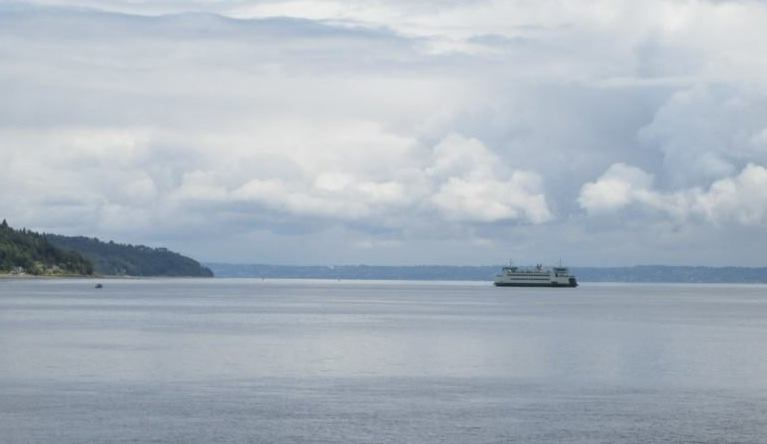
\includegraphics[scale = .55]{ferry2.jpg}
\end{center}
\end{figure}



\end{document}  